\documentclass[a4paper,12pt]{article}

\usepackage[utf8]{inputenc}
\usepackage[T1]{fontenc}
\usepackage{graphicx}
\usepackage{float}

\author{Antoine CARPENTIER}
\title{Heuristic optimization\\ \small Implementation exercises 2}

\bibliographystyle{apalike}

\begin{document}
\maketitle

\section{Exercise 1}

I implemented an \textit{iterated constructive greedy algorithm} and a \textit{genetic algorithm}. Both are parametrized by a run-time duration.

\subsection{Implementation}

\subsubsection{Iterated constructive greedy}

At each iteration the \textit{iterated constructive greedy algorithm} constructs a solution using an adapted cover greedy algorithm and performs a perturbative search with best improvement. It is inspired by \cite{resende2009greedy}. Bad solutions are discarded and a new solution is constructed.
I used those two algorithms because they are the most accurate.
The reason I implemented this "simple" algorithm is that it could reuse entirely the algorithms of implementation 1 and still have good results.

The function \texttt{iterated\_greedy} implements this algorithm.

\subsubsection{Genetic algorithm}

The \textit{genetic algorithm} is heavily inspired by \cite{beasley1996genetic}. 
It uses a population of size $ n * d $ where $ n $ is the number of subsets and $ d $ the density of the cover matrix. Having a big population helps escaping local minima but is very expensive in terms of time. The original idea used a coefficient more but it was too heavy and did not improve the results much.
The inital population is generated using \textit{random construction} and \textit{perturbative search with first improvement}. I chose the random construction for its speed and the perturbative search because it can improves a solution, if not well, at least quickly. 
The selection phase is handled using \textit{tournament selection} with a pool size of 10. I also tried \textit{proportional selection} but it was very slow and did not improve the solution. The pool size of 10 (they choose 2 in the paper) allows for more competition between individuals to evoluate quicker.
I use the \textit{generalised fitness-based} crossover operator from \cite{beasley1996genetic} to create one child by iteration.
The child is then mutated with a constant mutation rate of $ \frac{1}{population size} $. I reached good results without a variable mutation rate.
After mutation it uses \textit{adapted cover greedy construction} and \textit{redundancy elimination} to create non-redundant feasible solution.
The child then randomly replaces a parent with above than average cost. No child is included in the population if it is a duplicate of an already existing solution.

\subsection{Results}

The \textit{iterative greedy algorithm} obtains an average percentage deviation of 0.087 on all the instances using a run-time of 100 times the CH4 + FI. The run takes 162 seconds. This algorithm is somewhat very basic but it has the property of escaping local minima by randomization, which allows it to perform far better than greedy and perturbative algorithms.
0.06391166853212994


\subsubsection{Relative percentage deviation}


\begin{figure}[h]
   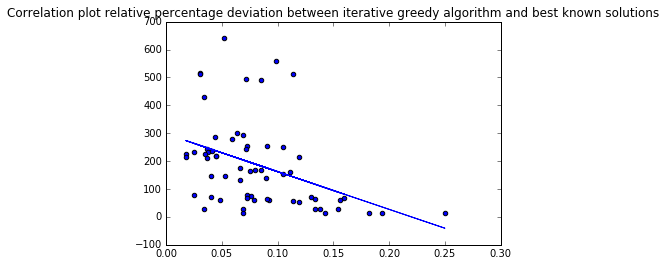
\includegraphics[width=\textwidth]{ig.png}
\end{figure}

\begin{figure}[h]
   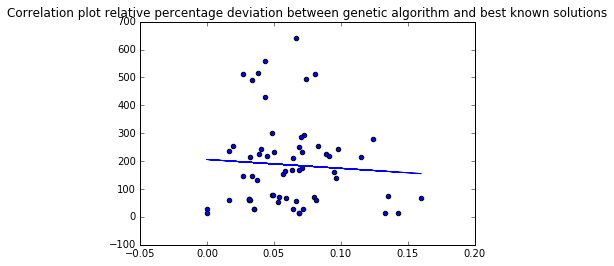
\includegraphics[width=\textwidth]{gen.png}
\end{figure}

\subsubsection{}

WilcoxonResult(statistic=446.0, pvalue=0.0015218128402173954)


\subsubsection{Optimum}



11.444749593734741
12.9664146900177
18.01086401939392
21.693324327468872
[258]
[78]
[234]
[61]

10.002309083938599
10.003480672836304
14.007994890213013
15.004057168960571
[272]
[81]
[235]
[63]


\bibliography{main}
\end{document}
